\chapter{Wie komplexe Zahlen Struktur erzeugen}
\label{chap:VII_komplexe Struktur}


\subsection{Iteration als mathematisches Prinzip}

\index{Iteration}
\index{Dynamisches System}
\index{Abbildung}

Iteration ist eines der einfachsten und zugleich mächtigsten Prinzipien der Mathematik:
Man nimmt eine Vorschrift, wendet sie an – und wendet das Ergebnis wieder auf dieselbe Vorschrift an.
Aus einer einzigen Regel entsteht eine Folge von Zuständen. Genau hier beginnt „Struktur aus Mathematik“.

Formal betrachtet ist Iteration die wiederholte Anwendung einer Abbildung $f$:
\[
z_{0},\quad z_{1}=f(z_{0}),\quad z_{2}=f(z_{1})=f(f(z_{0})),\quad \ldots,\quad z_{n+1}=f(z_n).
\]
Damit wird aus einer Zahl $z_0$ eine ganze Bahn durch den Zustandsraum.
\index{Orbit}

\subsubsection*{Ein wirkliches Zahlenbeispiel (damit das Schema greifbar wird)}
Nehmen wir eine extrem einfache Funktion auf den reellen Zahlen:
\[
f(x)=\frac12 x + 1.
\]
Wir starten mit $x_0=0$ und wenden immer wieder dieselbe Vorschrift an:
\[
\begin{aligned}
	x_1 &= f(x_0)=1,\\
	x_2 &= f(x_1)=1{,}5,\\
	x_3 &= f(x_2)=1{,}75,\\
	x_4 &= 1{,}875,\\
	x_5 &= 1{,}9375,\\
	x_6 &= 1{,}96875.
\end{aligned}
\]
Man sieht sofort: Die Folge nähert sich einer festen Zahl an, nämlich $2$.
Diese Zahl ist ein \emph{Fixpunkt}, denn $f(2)=2$ gilt.
\index{Fixpunkt}

\begin{DidacticBox}[Was man hier wirklich lernen soll]
	\index{Iteration}
	Iteration bedeutet nicht „eine Rechnung“, sondern \emph{eine Regel in der Zeit}:
	Aus $x_0$ wird $x_1$, daraus $x_2$, daraus $x_3$.
	Schon bei einer simplen Vorschrift entstehen typische Verhaltensweisen:
	\emph{Annäherung} (stabil), \emph{Schwanken} (periodisch) oder \emph{Weglaufen} (divergent).
\end{DidacticBox}

Diese Sicht ist entscheidend: Zahlen werden zu Zuständen, und die Funktion $f$ wird zur Dynamik.
Damit ist Iteration bereits ein dynamisches System – im reinsten, abstraktesten Sinn.
\index{Dynamisches System}

\begin{MathBox}[Begriffe: Orbit und Fixpunkt]
	\index{Orbit}
	\index{Fixpunkt}
	Gegeben sei $f:\mathbb{C}\to\mathbb{C}$ und ein Startwert $z_0\in\mathbb{C}$.
	Die Iteration ist
	\[
	z_{n+1}=f(z_n)\qquad (n=0,1,2,\dots).
	\]
	Die Folge $(z_0,z_1,z_2,\dots)$ heißt \emph{Orbit} (Bahn) von $z_0$.
	Ein Punkt $z^\ast$ heißt \emph{Fixpunkt}, wenn $f(z^\ast)=z^\ast$ gilt.
\end{MathBox}

\subsubsection*{Warum komplexe Zahlen hier etwas Besonderes sind}
\index{Komplexe Zahl}
\index{Komplexe Ebene}
In $\mathbb{R}$ läuft eine Iteration entlang einer Zahlengeraden. In $\mathbb{C}$ bewegt sie sich in einer Ebene.
Allein dieser Schritt verändert alles: Bahnen können kreisen, spiralförmig streben, Grenzen ausbilden,
Inseln erzeugen und feine Ränder entwickeln. Aus einer Vorschrift wird Geometrie.

Für die späteren Bilder (Mandelbrot- und Julia-Mengen) genügt im Kern eine einzige Familie:
\[
f_c(z)=z^2+c \qquad (z,c\in\mathbb{C}).
\]
Wir starten bei einem $z_0$ und verfolgen die Iteration. Die Leitfrage ist dabei brutal simpel:
\emph{Bleibt die Bahn beschränkt oder fliegt sie ins Unendliche?}

\subsubsection*{Kurzfazit}
\begin{itemize}
	\item Iteration heißt: dieselbe Vorschrift immer wieder anwenden.
	\item Das erzeugt Bahnen (Orbits) mit qualitativ verschiedenem Verhalten: stabil, periodisch oder divergent.
	\item In der komplexen Ebene wird dieses Verhalten sichtbar als Form.
\end{itemize}

\noindent\textbf{Übergang:} Im nächsten Abschnitt klären wir präzise, was „beschränkt“ und „divergent“ bedeutet
und warum genau der Grenzbereich zwischen beidem später die Struktur trägt.

\subsection{Stabilität, Divergenz und Grenzfälle}
\index{Stabilität}
\index{Divergenz}
\index{Grenzfall}
\index{Orbit}

Wenn wir eine Iteration $z_{n+1}=f(z_n)$ betrachten, dann ist die zentrale Frage nicht „Welche Zahl kommt als nächste?“,
sondern: \emph{Was passiert langfristig?}
Bleibt die Bahn in einem begrenzten Bereich, oder läuft sie davon?
Diese einfache Unterscheidung trennt stabile von instabilen Dynamiken.

\subsubsection*{Stabilität: Bahnen bleiben in der Nähe}
Im stabilen Fall ist ein Startwert „robust“: Kleine Änderungen am Startwert verändern zwar die Folge,
aber nicht ihr qualitatives Verhalten. Man kann sich das so vorstellen:
Die Iteration zieht Bahnen in einen bestimmten Bereich hinein, statt sie hinauszutreiben.
Typisch ist dabei die Annäherung an einen Fixpunkt oder an einen periodischen Zyklus.
\index{Fixpunkt}
\index{Periode}

\subsubsection*{Divergenz: Bahnen fliegen weg}
Im instabilen Fall passiert das Gegenteil: Die Iteration verstärkt Abweichungen.
Die Folge wächst im Betrag immer weiter, sie „entkommt“ aus jedem beschränkten Bereich.
Genau dieses Verhalten werden wir später als Kriterium verwenden: \emph{Wer wegfliegt, gehört nicht zur Struktur.}
\index{Betrag}
\subsubsection*{Zwei Mini-Beispiele: stabil vs.\ divergent}
\index{Stabilität}
\index{Divergenz}

\begin{figure}[h]
	\centering
	
	\begin{tikzpicture}
		\begin{axis}[
			width=0.46\textwidth,
			height=4.2cm,
			xlabel={$n$},
			ylabel={$x_n$},
			title={Stabil: $x_{n+1}=\tfrac12 x_n+1$},
			ymin=0, ymax=2.1,
			xtick={0,1,2,3,4,5,6,7,8},
			ytick={0,0.5,1,1.5,2}
			]
			\addplot+[mark=*] coordinates {
				(0,0)
				(1,1)
				(2,1.5)
				(3,1.75)
				(4,1.875)
				(5,1.9375)
				(6,1.96875)
				(7,1.984375)
				(8,1.9921875)
			};
		\end{axis}
	\end{tikzpicture}
	\hfill
	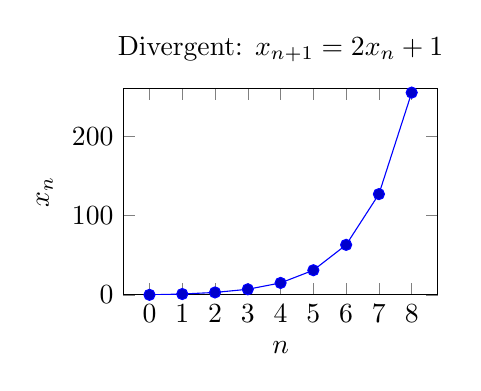
\begin{tikzpicture}
		\begin{axis}[
			width=0.46\textwidth,
			height=4.2cm,
			xlabel={$n$},
			ylabel={$x_n$},
			title={Divergent: $x_{n+1}=2x_n+1$},
			ymin=0, ymax=260,
			xtick={0,1,2,3,4,5,6,7,8}
			]
			\addplot+[mark=*] coordinates {
				(0,0)
				(1,1)
				(2,3)
				(3,7)
				(4,15)
				(5,31)
				(6,63)
				(7,127)
				(8,255)
			};
		\end{axis}
	\end{tikzpicture}
	
\end{figure}
\begin{DidacticBox}[Stabil vs.\ chaotisch: nicht verwechseln]
	\index{Chaos}
	Stabilität bedeutet nicht „langweilig“, und Instabilität bedeutet nicht automatisch „Zufall“.
	Auch chaotische Bahnen sind deterministisch, aber sie sind empfindlich gegenüber kleinsten Änderungen.
	Für unsere Zwecke reicht zunächst eine robustere Leitidee:
	\emph{beschränkt} versus \emph{unbeschränkt}.
	Der Grenzbereich zwischen beidem ist später der Ort der sichtbaren Struktur.
\end{DidacticBox}

\subsubsection*{Beschränktheit als Kriterium}
In der komplexen Ebene ist es besonders natürlich, den \emph{Betrag} $|z_n|$ zu betrachten.
Wir nennen einen Orbit \emph{beschränkt}, wenn es eine Zahl $R>0$ gibt, so dass
\[
|z_n|\le R \quad \text{für alle } n.
\]
Existiert kein solches $R$, dann läuft der Orbit ins Unendliche: $|z_n|\to\infty$.

\begin{MathBox}[Beschränkt oder unbeschränkt]
	\index{Beschränktheit}
	\index{Betrag}
	Für die Iteration $z_{n+1}=f(z_n)$ heißt der Orbit von $z_0$ \emph{beschränkt}, wenn
	\[
	\exists\, R>0:\ \forall n\in\mathbb{N}\ \ |z_n|\le R.
	\]
	Ist das nicht der Fall, nennt man den Orbit \emph{unbeschränkt} (oder divergent);
	typisch ist dann $|z_n|\to\infty$.
\end{MathBox}
\subsubsection*{Ein einfaches komplexes Beispiel: Spiralbahn im Kreis}
Wir betrachten die Iteration
\[
z_{n+1}=a\,z_n,\qquad a=0{,}85\,e^{i\pi/5},\qquad z_0=2+i.
\]
Da $|a|=0{,}85<1$ gilt
\[
|z_n|=|a|^n|z_0|\le |z_0|=:R=\sqrt{5}.
\]
Der Orbit bleibt also für alle $n$ im Kreisradius $R$ und spiralt gegen $0$.

\begin{figure}[h]
	\centering
	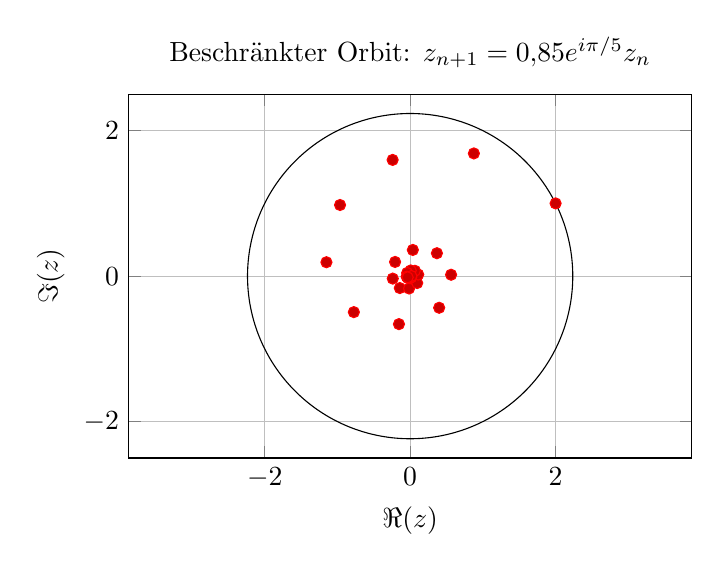
\begin{tikzpicture}
		\begin{axis}[
			axis equal,
			width=0.72\textwidth,
			height=6.2cm,
			xlabel={$\Re(z)$},
			ylabel={$\Im(z)$},
			title={Beschränkter Orbit: $z_{n+1}=0{,}85e^{i\pi/5}z_n$},
			xmin=-2.5, xmax=2.5,
			ymin=-2.5, ymax=2.5,
			grid=both
			]
			% Kreisradius R = sqrt(5)
			\addplot[domain=0:360, samples=361] ({sqrt(5)*cos(x)},{sqrt(5)*sin(x)});
			
			% Orbitpunkte (n=0..25)
			\addplot+[only marks, mark=*] coordinates {
				(2.000,1.000)
				(0.876,1.687)
				(-0.241,1.598)
				(-0.964,0.978)
				(-1.151,0.191)
				(-0.774,-0.495)
				(-0.154,-0.660)
				(0.399,-0.435)
				(0.563,0.019)
				(0.368,0.315)
				(0.037,0.360)
				(-0.207,0.195)
				(-0.239,-0.034)
				(-0.142,-0.164)
				(-0.015,-0.170)
				(0.097,-0.095)
				(0.111,0.022)
				(0.066,0.073)
				(0.008,0.078)
				(-0.041,0.044)
				(-0.048,-0.007)
				(-0.030,-0.026)
				(-0.005,-0.028)
				(0.015,-0.016)
				(0.017,0.002)
				(-0.034,-0.017)
			};
		\end{axis}
	\end{tikzpicture}
\end{figure}
\subsubsection*{Der Grenzfall: die eigentliche Bühne der Struktur}
Jetzt kommt der entscheidende Punkt für das ganze Kapitel:
Zwischen eindeutig stabil und eindeutig divergent liegt ein Randbereich, der extrem empfindlich ist.
Startwerte, die nur minimal voneinander abweichen, können völlig verschieden enden:
Der eine Orbit bleibt beschränkt, der andere fliegt weg.
Dieser „Übergang“ ist kein Nebeneffekt, sondern das Zentrum des Phänomens.

Genau deshalb entstehen später scharfe, fransige Grenzen und scheinbar unendliche Detailtiefe.
Nicht weil wir Natur modellieren, sondern weil wir eine mathematische Grenzfrage stellen.
\subsubsection*{Grenzfall: eine minimale Änderung entscheidet alles}
Wir betrachten die Iteration
\[
z_{n+1}=z_n^2,
\]
also die Quadratik $f(z)=z^2$. Hier lässt sich der Grenzfall vollständig verstehen:
\emph{Die Grenze zwischen beschränkt und unbeschränkt ist der Einheitskreis $|z|=1$.}
Damit ist bereits sichtbar, was später bei Mandelbrot- und Julia-Mengen in viel komplizierterer Form auftritt:
Ein Randbereich entscheidet über „bleibt drin“ oder „fliegt weg“.

Wir wählen zwei fast identische Startwerte:
\[
z_0=0{,}99 \quad (\text{knapp innerhalb}), 
\qquad z_0=1{,}01 \quad (\text{knapp außerhalb}).
\]

\begin{figure}[h]
	\centering
	
	% --- Bild links: komplexe Ebene mit Einheitskreis und Startpunkten ---
	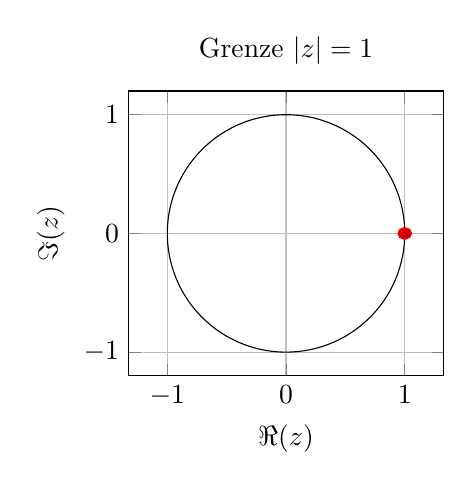
\begin{tikzpicture}
		\begin{axis}[
			axis equal,
			width=0.46\textwidth,
			height=5.2cm,
			xlabel={$\Re(z)$},
			ylabel={$\Im(z)$},
			title={Grenze $|z|=1$},
			xmin=-1.2, xmax=1.2,
			ymin=-1.2, ymax=1.2,
			grid=both
			]
			% Einheitskreis
			\addplot[domain=0:360, samples=361] ({cos(x)},{sin(x)});
			% Startpunkte
			\addplot+[only marks, mark=*] coordinates {(0.99,0) (1.01,0)};
		\end{axis}
	\end{tikzpicture}
	\hfill
	% --- Bild rechts: Betrag als Funktion von n (log-Skala) ---
	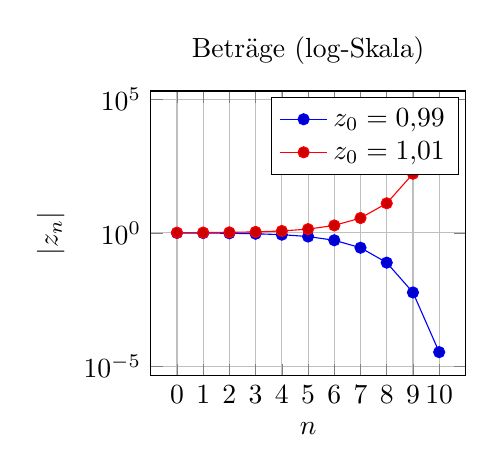
\begin{tikzpicture}
		\begin{axis}[
			width=0.46\textwidth,
			height=5.2cm,
			xlabel={$n$},
			ylabel={$|z_n|$},
			title={Beträge (log-Skala)},
			ymode=log,
			log basis y={10},
			xtick={0,1,2,3,4,5,6,7,8,9,10},
			grid=both
			]
			% z0=0.99
			\addplot+[mark=*] coordinates {
				(0,0.99)
				(1,0.9801)
				(2,0.96059601)
				(3,0.9227446944)
				(4,0.8514577711)
				(5,0.7249803360)
				(6,0.5255964875)
				(7,0.2762516677)
				(8,0.0763149839)
				(9,0.0058239768)
				(10,0.0000339187)
			};
			\addlegendentry{$z_0=0{,}99$}
			
			% z0=1.01
			\addplot+[mark=*] coordinates {
				(0,1.01)
				(1,1.0201)
				(2,1.04060401)
				(3,1.0828567056)
				(4,1.1725786449)
				(5,1.3749406785)
				(6,1.8904618695)
				(7,3.5738460800)
				(8,12.7723758032)
				(9,163.1335836586)
				(10,26612.5661173053)
			};
			\addlegendentry{$z_0=1{,}01$}
		\end{axis}
	\end{tikzpicture}
	
	\caption{Grenzfall bei $z_{n+1}=z_n^2$: Innerhalb des Einheitskreises bleiben Bahnen beschränkt, außerhalb divergieren sie. Schon eine minimale Änderung des Startwerts kann das Verhalten vollständig kippen.}
\end{figure}
\subsubsection*{Vorbereitung auf die Quadratik $z^2+c$}
\index{Quadratische Abbildung}
Für die Familie $f_c(z)=z^2+c$ wird es sogar ein praktisches Kriterium geben:
Wenn der Betrag eines Orbit irgendwann groß genug wird, dann ist sicher, dass er weiter wächst und entkommt.
Damit lässt sich „dazugehörig“ versus „nicht dazuzugehörig“ rechnerisch entscheiden.

\noindent\textbf{Übergang:} Im nächsten Abschnitt verwenden wir genau diese Idee als Landkarte:
Für welche Parameter $c$ bleibt der Orbit von $z_0=0$ beschränkt?
Die Antwort ist die Mandelbrot-Menge.






\subsection{Die Mandelbrot-Menge als Landkarte}
Kant

\subsection{Julia-Mengen: lokale Dynamik und Struktur}
Heu
\subsection{Selbstähnlichkeit und Skaleninvarianz}
He

\subsection{Warum diese Formen keine Naturmodelle sind}
Heute

\subsection{	Fazit: Struktur ohne Materie}
Heut